\begin{figure}[htbp]
    \centering
    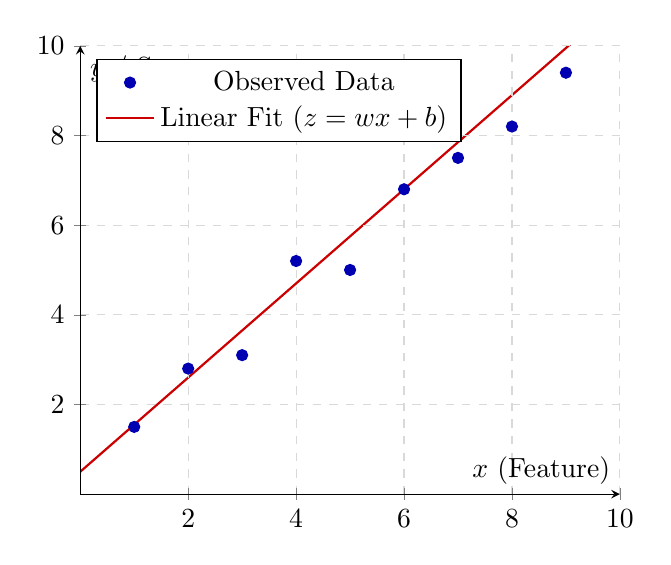
\begin{tikzpicture}
        \begin{axis}[
            xlabel={$x$ (Feature)},
            ylabel={$y$ / Score $z$},
            xmin=0, xmax=10,
            ymin=0, ymax=10,
            axis lines=center,
            axis on top=true,
            grid=major,
            grid style={dashed, gray!30},
            legend pos=north west
        ]
            % Punti del dataset (osservazioni reali)
            \addplot[only marks, mark=*, blue!70!black] coordinates {
                (1, 1.5) (2, 2.8) (3, 3.1) (4, 5.2) (5, 5.0) 
                (6, 6.8) (7, 7.5) (8, 8.2) (9, 9.4)
            };
            
            % Retta di regressione (il modello lineare: z = w*x + b)
            \addplot[domain=0:10, red!80!black, thick] {1.05 * x + 0.5};
            
            \legend{Observed Data, Linear Fit ($z = wx + b$)}
        \end{axis}
    \end{tikzpicture}
    \caption{Geometric representation of 2D linear regression.}
    \label{fig:linear_regression_2d}
\end{figure}